\let\negmedspace\undefined
\let\negthickspace\undefined
\documentclass[journal]{IEEEtran}
\usepackage[a5paper, margin=10mm, onecolumn]{geometry}
\usepackage{lmodern} % Ensure lmodern is loaded for pdflatex
\usepackage{tfrupee} % Include tfrupee package

\setlength{\headheight}{1cm} % Set the height of the header box
\setlength{\headsep}{0mm}     % Set the distance between the header box and the top of the text

\usepackage{gvv-book}
\usepackage{gvv}
\usepackage{cite}
\usepackage{amsmath,amssymb,amsfonts,amsthm}
\usepackage{algorithmic}%lflfls
\usepackage{graphicx}
\graphicspath{{./figs/}}
\usepackage{textcomp}
\usepackage{xcolor}
\usepackage{txfonts}
\usepackage{listings}
\usepackage{enumitem}
\usepackage{mathtools}
\usepackage{gensymb}
\usepackage{comment}
\usepackage[breaklinks=true]{hyperref}
\usepackage{tkz-euclide} 
\usepackage{listings}
\usepackage{gvv}                                        
\def\inputGnumericTable{}                                 
\usepackage[latin1]{inputenc}                                
\usepackage{color}                                            
\usepackage{array}                                            
\usepackage{longtable}                                       
\usepackage{calc}                                             
\usepackage{multirow}                                         
\usepackage{hhline}                                           
\usepackage{ifthen}                                           
\usepackage{lscape}
\usepackage{circuitikz}
\tikzstyle{block} = [rectangle, draw, fill=blue!20, 
text width=4em, text centered, rounded corners, minimum height=3em]
\tikzstyle{sum} = [draw, fill=blue!10, circle, minimum size=1cm, node distance=1.5cm]
\tikzstyle{input} = [coordinate]
\tikzstyle{output} = [coordinate]


\begin{document}
	
	\bibliographystyle{IEEEtran}
	\vspace{3cm}
	
	\title{2.8.24}
	\author{EE25BTECH11042 - Nipun Dasari}
	\maketitle
	% \newpage
	% \bigskip
	{\let\newpage\relax\maketitle}
	
	\renewcommand{\thefigure}{\theenumi}
	\renewcommand{\thetable}{\theenumi}
	\setlength{\intextsep}{10pt} % Space between text and floats
	
	
	\numberwithin{equation}{enumi}
	\numberwithin{figure}{enumi}
	\renewcommand{\thetable}{\theenumi}
	
	\textbf{Question}:\\
	The $\vec{a} + \vec{b}$ bisects the angle between $\vec{a}$ and $\vec{b}$ if \underline{\hspace{2cm}}
	
	\solution \\
	Theorem: The $\vec{a} + \vec{b}$ bisects the angle between $\vec{a}$ and $\vec{b}$ if and only if $\norm{\vec{a}}$ = $\norm{\vec{b}}$ \\
	We prove the above in two parts:\\
	Assume a $\vec{c}$ such that
	\begin{align}
		\vec{c} = \vec{a} + \vec{b} \label{0.2}
	\end{align}
	Let $\alpha$ and $\beta$ be angles made by $\vec{c}$ with $\vec{a}$ and $\vec{b}$ respectively.\\
	\textbf{Part 1}\\
	Given : 
	\begin{align}
		\norm{\vec{a}} = \norm{\vec{b}} \label{0.1}
	\end{align}
	To prove : $\vec{a} + \vec{b}$ bisects the angle between $\vec{a}$ and $\vec{b}$\\
	Proof: \\	
	The angle $\theta$ between $\vec{p}$ and $\vec{q}$ is given by: 
	\begin{align}
		\cos\theta = \frac{\vec{p}^\top\vec{q}}{\norm{\vec{p}}\norm{\vec{q}}} \label{0.3}
	\end{align}
	By \eqref{0.3} and \eqref{0.2}
	\begin{align}
		\implies \cos\alpha = \frac{\vec{a}^\top\brak{\vec{a}+\vec{b}}}{\norm{\vec{a}}\norm{\vec{a}+\vec{b}}} 
	\end{align}
	\begin{align}
		\implies \cos\beta = \frac{\vec{b}^\top\brak{\vec{a}+\vec{b}}}{\norm{\vec{b}}\norm{\vec{a}+\vec{b}}} 
	\end{align}
	By \eqref{0.1}
	\begin{align}
		\vec{a}^\top\vec{a} = \vec{b}^\top\vec{b}
	\end{align}
	\begin{align}
		\vec{a}^\top\vec{a} + \vec{a}^\top\vec{b} = \vec{b}^\top\vec{b} + \vec{b}^\top\vec{a}
	\end{align}
	\begin{align}
\frac{\vec{a}^\top\vec{a} + \vec{a}^\top\vec{b}}{\norm{\vec{a}}\norm{\vec{a}+\vec{b}}} = \frac{\vec{b}^\top\vec{b} + \vec{b}^\top\vec{a}}{\norm{\vec{b}}\norm{\vec{a}+\vec{b}}}
	\end{align}
	\begin{align}
	\therefore \cos\alpha=	\cos\beta   \label{angle}
	\end{align}	
	\begin{align}
	\therefore	\alpha=\beta
	\end{align}	
	\textbf{Part 2}\\
	Given:
	\begin{align}
		\alpha=\beta
	\end{align}
	To prove:
	\begin{align}
		\norm{\vec{a}} = \norm{\vec{b}} 
	\end{align}
	Proof:\\
	By \eqref{angle}
	\begin{align}
		\cos{\alpha}=\cos{\beta}
	\end{align}
	\begin{align}
		\frac{\vec{a}^\top\brak{\vec{a}+\vec{b}}}{\norm{\vec{a}}\norm{\vec{a}+\vec{b}}} = \frac{\vec{b}^\top\brak{\vec{a}+\vec{b}}}{\norm{\vec{b}}\norm{\vec{a}+\vec{b}}}
	\end{align}
\begin{align}
	\norm{\vec{b}} (\norm{\vec{a}}^2 + \vec{a}^\top\vec{b}) = \norm{\vec{a}} (\norm{\vec{b}}^2 + \vec{a}^\top\vec{b}) \\
	\norm{\vec{b}}\norm{\vec{a}}^2 + \norm{\vec{b}}(\vec{a}^\top\vec{b}) = \norm{\vec{a}}\norm{\vec{b}}^2 + \norm{\vec{a}}(\vec{a}^\top\vec{b})
\end{align}

Rearrange the terms to group common factors:
\begin{align}
	\norm{\vec{b}}\norm{\vec{a}}^2 - \norm{\vec{a}}\norm{\vec{b}}^2 = \norm{\vec{a}}(\vec{a}^\top\vec{b}) - \norm{\vec{b}}(\vec{a}^\top\vec{b})
\end{align}
\begin{align}
	\norm{\vec{a}}\norm{\vec{b}} (\norm{\vec{a}} - \norm{\vec{b}}) = (\vec{a}^\top\vec{b}) (\norm{\vec{a}} - \norm{\vec{b}})
\end{align}

\begin{align}
	(\norm{\vec{a}} - \norm{\vec{b}}) (\norm{\vec{a}}\norm{\vec{b}} - \vec{a}^\top\vec{b}) = 0
\end{align}

This equation gives two possibilities:
\begin{align}
	\norm{\vec{a}} - \norm{\vec{b}} = 0 \implies \norm{\vec{a}} = \norm{\vec{b}}\\
	\norm{\vec{a}}\norm{\vec{b}} - \vec{a}^\top\vec{b} = 0 \implies \vec{a}^\top\vec{b} = \norm{\vec{a}}\norm{\vec{b}}\text{} \label{np}
\end{align}
\eqref{np} is incorrect as parallel vectors are not being assumed.\\
Thus proved
	
	
	
		\begin{figure}[H]
		\centering
		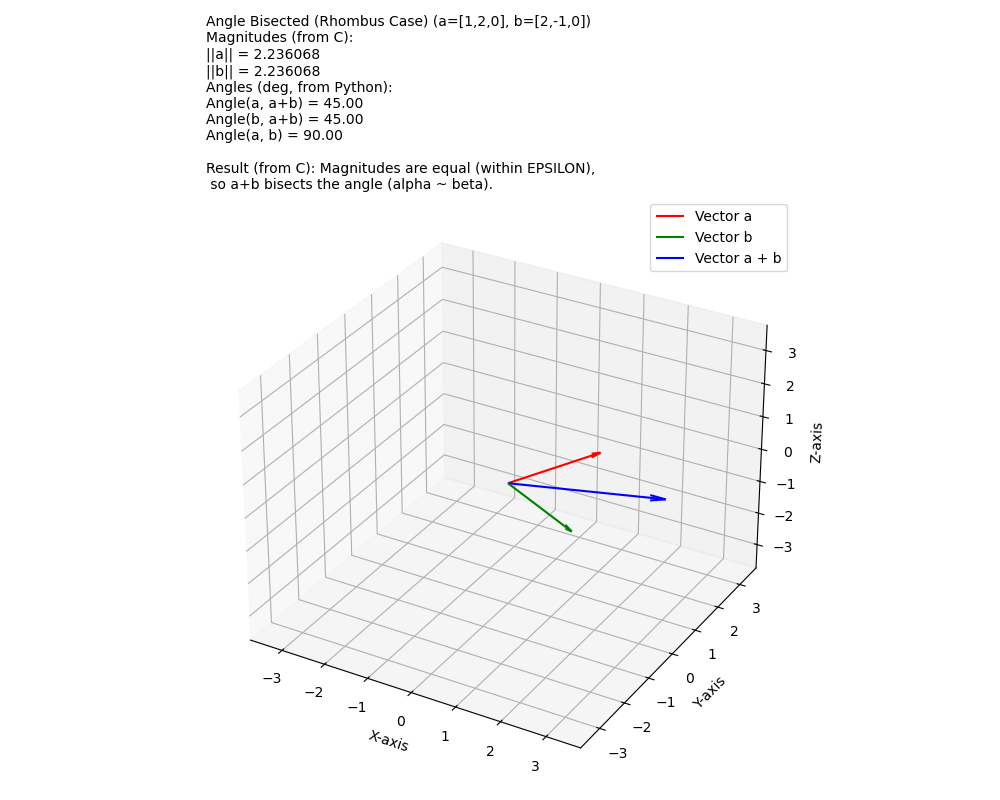
\includegraphics[width = 0.6\columnwidth]{Figure_1.png}
		\caption*{}
		\label{fig1}
	\end{figure}
	\begin{figure}[H]
		\centering
		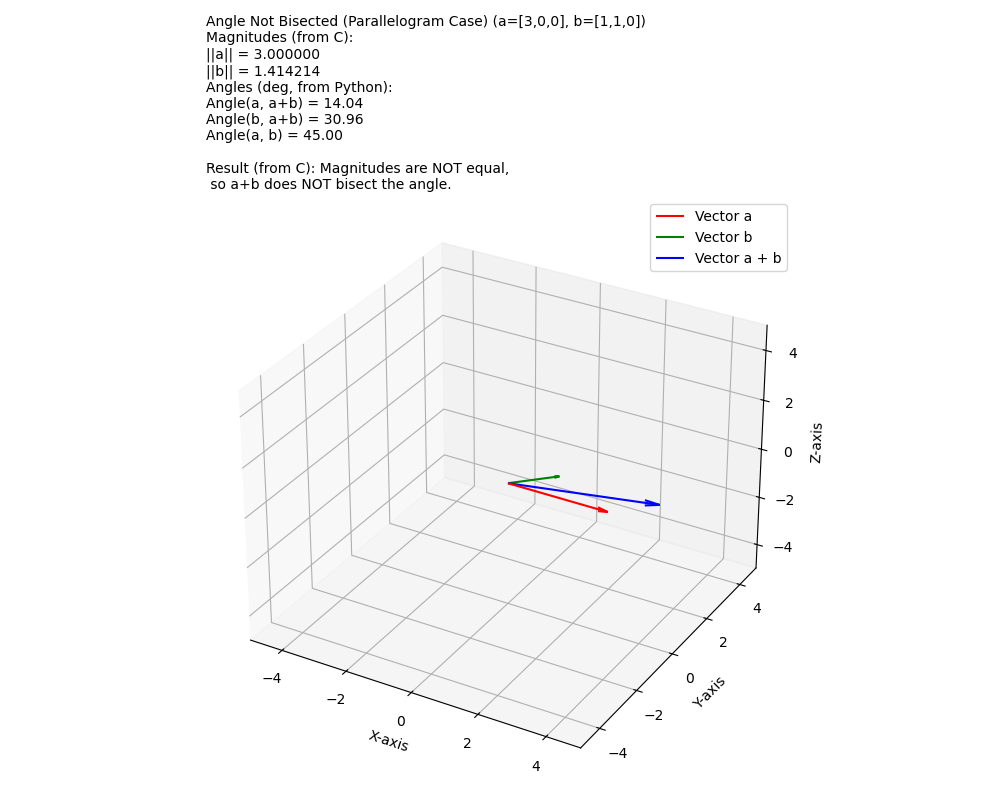
\includegraphics[width = 0.6\columnwidth]{Figure_2.png}
		\caption*{}
		\label{fig2}
	\end{figure}
	
	
\end{document}